\section{Results and Discussion}\label{sec:results}

This section reports the historical cached runs with the unit weight $\rho=1$; Section~\ref{sec:rho} compares them with the runs under the
bit-level weight $\rho_K$. Both costs are computed from model structures; neither uses measured energy. The corrected-study comparisons remain in their separate reports and are not combined with these historical numbers.

\begin{table*}[!htbp]
\centering
\caption{Results over 30 independent runs with $\rho=1$: median [interquartile range]. HV: hypervolume of the delivered set (identification or free-run validation error); $C_\tau$, NRMSE$_\tau$: cost and free-run validation NRMSE of the model selected by the $\tau$-rule; Rec.$_\tau$, Rec.$_\mathcal{P}$: fraction of runs in which the selected model, or at least one model of the returned set, contains the three true regressors of \eqref{eq:tutorial}. $^{\ast}$/$^{\dagger}$: Green differs from SO/MO-lex (Mann--Whitney, Holm-adjusted $p<0.05$).}
\label{tab:results}
\footnotesize
\setlength{\tabcolsep}{2.5pt}
\resizebox{\textwidth}{!}{%
\begin{tabular}{llcccccc}
\toprule
Ex. & Method & HV$_\mathrm{id}$ & HV$_\mathrm{val}$ & $C_\tau$ & NRMSE$_\tau$ & Rec.$_\tau$ & Rec.$_\mathcal{P}$ \\
\midrule
\multirow{3}{*}{E1} & SO & 0.640 [0.560, 0.640] & 0.640 [0.560, 0.640] & 9 [9, 11] & 3e-16 [2e-16, 3e-16] & 1.00 & 1.00 \\
 & MO-lex & 0.829 [0.803, 0.829] & 0.827 [0.798, 0.827] & 7 [7, 7] & 3e-16 [3e-16, 3e-16] & 1.00 & 1.00 \\
 & \textbf{Green} & 0.896 [0.896, 0.896]$^{\ast}$$^{\dagger}$ & 0.893 [0.893, 0.893]$^{\ast}$$^{\dagger}$ & 7 [7, 7]$^{\ast}$ & 9e-16 [7e-16, 2e-15]$^{\ast}$$^{\dagger}$ & 1.00 & 1.00 \\
\midrule
\multirow{3}{*}{E2} & SO & 0.508 [0.508, 0.508] & 0.505 [0.505, 0.505] & 12 [12, 12] & 0.028 [0.028, 0.028] & 0.00 & 0.00 \\
 & MO-lex & 0.702 [0.661, 0.703] & 0.699 [0.656, 0.700] & 10 [9, 10] & 0.028 [0.028, 0.029] & 0.00 & 0.07 \\
 & \textbf{Green} & 0.878 [0.878, 0.879]$^{\ast}$$^{\dagger}$ & 0.872 [0.872, 0.874]$^{\ast}$$^{\dagger}$ & 7 [7, 7]$^{\ast}$$^{\dagger}$ & 0.028 [0.028, 0.028] & 0.00 & 0.00 \\
\midrule
\multirow{3}{*}{E3} & SO & 0.736 [0.729, 0.770] & 0.000 [0.000, 0.000] & 18.5 [16, 19] & 1.394 [1.301, 1.463] & -- & -- \\
 & MO-lex & 0.798 [0.797, 0.825] & 0.000 [0.000, 0.471] & 16 [16, 16] & 1.411 [1.340, 1.467] & -- & -- \\
 & \textbf{Green} & 0.955 [0.932, 0.956]$^{\ast}$$^{\dagger}$ & 0.893 [0.868, 0.893]$^{\ast}$$^{\dagger}$ & 16 [14.5, 16]$^{\ast}$ & 1.420 [1.316, 1.451] & -- & -- \\
\bottomrule
\end{tabular}}
\end{table*}


\subsection{Quality of the trade-off sets}
Table~\ref{tab:results} summarises the \nSeeds{} runs per configuration. On all three examples, Green MGGP returns
sets with higher hypervolume than both baselines, in identification (\EBGreenHVid, \ECGreenHVid{} and \EDGreenHVid{}
against \EBLexHVid, \ECLexHVid{} and \EDLexHVid{} for MO-lex) and in free-run validation (\EBGreenHVval, \ECGreenHVval{}
and \EDGreenHVval{} against \EBLexHVval, \ECLexHVval{} and \EDLexHVval). Every Green run exceeds every baseline run on
these indicators with the declared reference $(1,1)$ ($A_{12}=1.00$, Holm-adjusted $p<10^{-8}$ for all twelve comparisons), and the Green interquartile
ranges are also the narrowest (Fig.~\ref{fig:hv}). The validation hypervolumes closely follow the identification
ones, so the additional low-cost models found by Green MGGP are not artefacts of the identification criterion.

\begin{figure}[t]
\centering
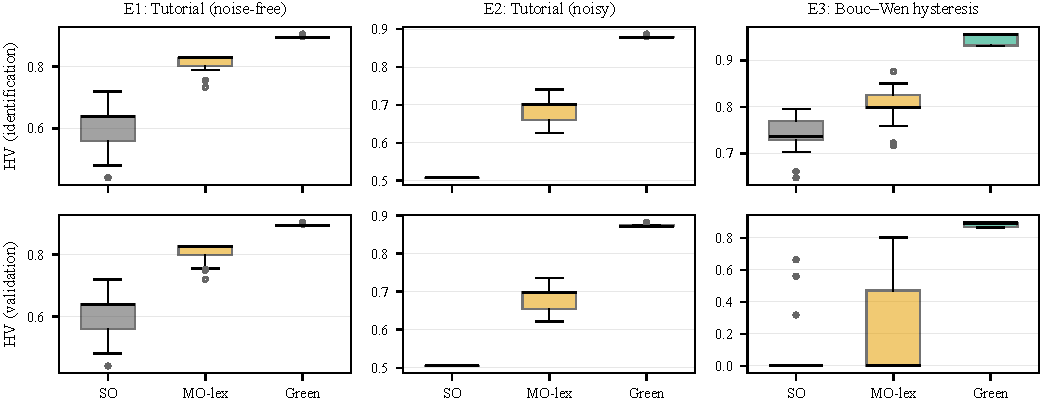
\includegraphics[width=\textwidth]{figures/fig_hv.pdf}
\caption{Hypervolume of the returned sets over \nSeeds{} runs with $\rho=1$, computed with the identification error
(top) and the free-run validation error (bottom) of the same models.}
\label{fig:hv}
\end{figure}

The SO comparison concerns its delivered single model, whereas MO-lex and Green return sets. As a diagnostic, the median identification hypervolume of the non-dominated final SO population is \ReviewEBSOPopHV, \ReviewECSOPopHV{} and \ReviewEDSOPopHV on E1--E3, close to MO-lex. This separates the effect of final filtering from the search itself without changing the declared SO output.

The complete separation of hypervolumes is conditional on the declared reference. Reference-point specification affects the relative contributions of different regions of a trade-off set~\cite{Ishibuchi2018}. Table~\ref{tab:hv_reference} recomputes validation hypervolume from the stored models with tighter error references, as a post-hoc sensitivity analysis. On E3, the Green--MO-lex effect approaches equality at an error reference of 0.1. Thus the primary indicator rewards the broad accuracy--cost trade-off, and does not establish superiority within every restricted high-accuracy region.
\begin{table}[!htbp]\centering
\caption{Post-hoc sensitivity of validation hypervolume to its error reference ($\rho=1$). $A_{12}$ compares Green with MO-lex; the cost reference is unchanged.}
\label{tab:hv_reference}
\begin{tabular}{lrrr}\toprule
Example & Error reference & Green median & $A_{12}$ \\ \midrule
E1 & 1 & 0.893 & 1.00 \\
E1 & 0.2 & 0.157 & 1.00 \\
E1 & 0.1 & 0.071 & 1.00 \\
E2 & 1 & 0.871 & 1.00 \\
E2 & 0.2 & 0.135 & 1.00 \\
E2 & 0.1 & 0.051 & 0.95 \\
E3 & 1 & 0.897 & 1.00 \\
E3 & 0.2 & 0.129 & 0.81 \\
E3 & 0.1 & 0.034 & 0.52 \\
\bottomrule\end{tabular}\end{table}


The hypervolume condenses each set into one number; Fig.~\ref{fig:attainment} shows where the differences lie. For
each run $r$ and cost level $c$, let $A_r(c)$ be the smallest error among the returned models with $C\le c$; the
figure shows the median and the interquartile band of $A_r(c)$ over the runs, that is, the 50\% empirical attainment
surface and its quartiles, following the attainment-based assessment of stochastic multi-objective optimisers~\cite{FF1996}. On E1, Green MGGP and MO-lex reach an exact model at the smallest reachable cost
in the median run, whereas SO needs a more expensive one, and beyond that cost the surfaces differ only at machine
precision. On E2, the surfaces of SO and MO-lex lie marginally below that of Green MGGP in
identification at costs between $12$ and $14$ (median NRMSE $0.0255$ against $0.0256$), but not in validation, where
the Green surface is the lowest at every cost. On E3 the picture is more nuanced: at costs of $18$ operations and
above, SO and MO-lex attain a lower identification error than Green MGGP, which spreads its population over the whole
cost axis instead of concentrating it at the expensive end. This advantage does not carry over to free-run
validation, where the Green surface is the lowest at every cost and reaches its smallest median validation error with
models of about $20$ operations. The baselines thus spend their budget refining expensive models whose additional
identification accuracy is not reflected in simulation.

\begin{figure}[t]
\centering
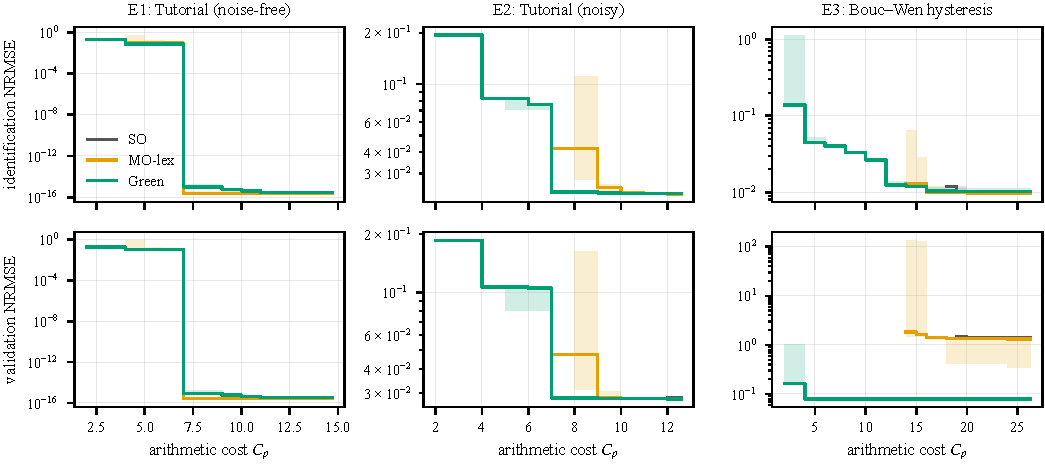
\includegraphics[width=\textwidth]{figures/fig_attainment.pdf}
\caption{Empirical attainment surfaces of the returned sets with $\rho=1$: median (lines) and interquartile band
(shading) over \nSeeds{} runs of the smallest identification error (top) and free-run validation error (bottom)
achieved within each cost budget. Logarithmic error axes; on E1 the errors are at machine precision once the exact
structure is reached.}
\label{fig:attainment}
\end{figure}

Fig.~\ref{fig:fronts} shows the sets behind these statistics for one representative run of each method, chosen by
the rule used throughout, the median validation error of the selected model. The Green sets cover the whole cost
range with many models: on E3, nine models between $2$ and $18$ operations per sample, against six models between $13$
and $21$ for MO-lex and a single model of $21$ operations for SO, and on E2 seven models between $2$ and $12$, against
four for MO-lex. In validation, the representative Green sets also contain the most accurate model of the three runs,
with NRMSE $0.0295$ at $9$ operations on E2 and $0.0617$ at $16$ operations on E3. On E3 the $\tau$-rule selects
instead the Green model of $18$ operations, whose validation error is $0.0787$, which illustrates on a single run the
limitation of a rule based on identification error alone.

\begin{figure}[t]
\centering
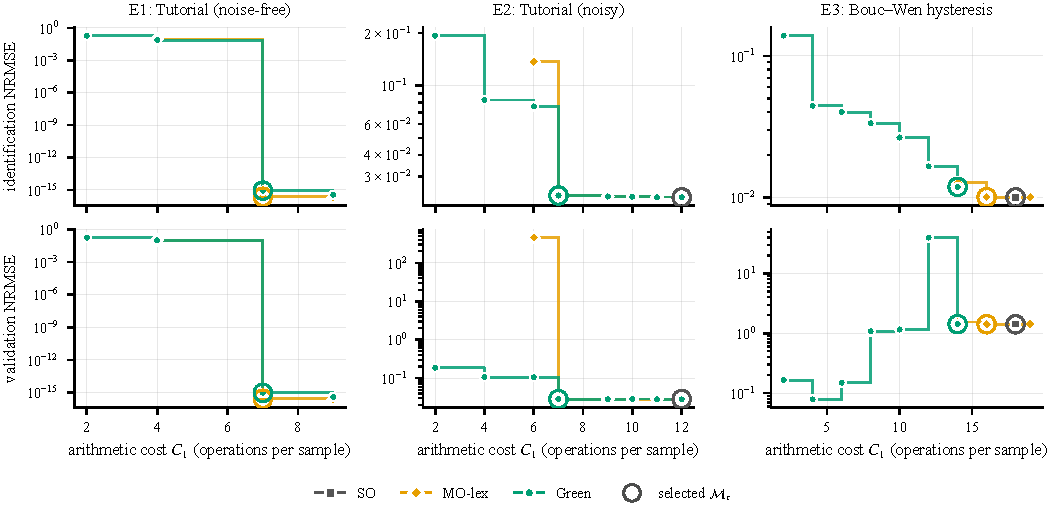
\includegraphics[width=\textwidth]{figures/fig_fronts.pdf}
\caption{Returned sets of the representative runs with $\rho=1$ (median validation error of the selected model; seeds
2, 27 and 15 on E1, 3, 26 and 2 on E2, and 22, 27 and 24 on E3, for SO, MO-lex and Green MGGP), plotted against the
identification error (top) and the free-run validation error of the same models (bottom). Rings mark the model
selected by the $\tau$-rule; errors below $10^{-16}$ are shown at $10^{-16}$.}
\label{fig:fronts}
\end{figure}

\subsection{Search dynamics and empirical verification of the theory}
Fig.~\ref{fig:convergence} follows the population of each run over the generations. Its top row shows the
hypervolume of the non-dominated subset of the population, with the cost of SO individuals computed \emph{a
posteriori}. For Green MGGP this quantity never decreases, as Theorem~\ref{thm:elitism} predicts, and it rises in
steps as cheaper or more accurate structures are found. For SO and MO-lex it peaks within the first few generations
and then decreases or oscillates, because elitism by error discards cheap non-dominated individuals once more
accurate ones appear. The two baseline curves are almost indistinguishable, as anticipated by
Theorem~\ref{thm:lex}. The bottom row shows the number of distinct structures in the population: with structural
duplicate removal, Green MGGP reaches $\mu=100$ distinct structures within two generations and keeps them, whereas
the median baseline populations hold between about $30$ and $80$, the rest being copies.

\begin{figure}[t]
\centering
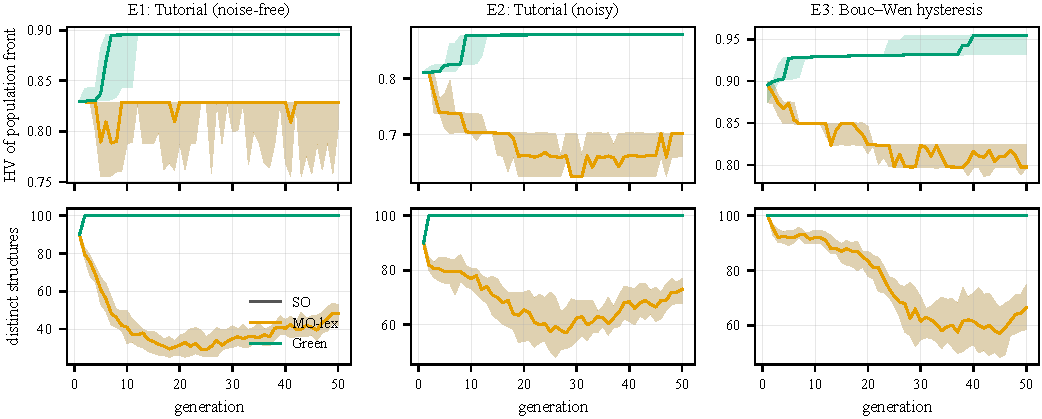
\includegraphics[width=\textwidth]{figures/fig_convergence.pdf}
\caption{Search dynamics with $\rho=1$: median (lines) and interquartile band (shading) over \nSeeds{} runs of the
hypervolume of the population front (top; for SO the cost is computed a posteriori) and of the number of distinct
structures in the population (bottom).}
\label{fig:convergence}
\end{figure}

\begin{table}[!htbp]
\centering
\caption{Empirical verification of Theorems~2 and~3 over 30 seeds. Lexicographic reduction: seeds in which SO and MO-lex produce identical populations in all generations; diverging seeds in which the divergence is preceded by an error tie between individuals of different cost, and in which the populations involved contain at least two individuals with $J_E=\infty$; median generation of the first divergence. Non-deterioration: largest $|U_t^1|$ over all runs and generations, bound $L(G,h)$ and population size $\mu$; runs with at least one decrease of the population-front hypervolume.}
\label{tab:checks}
\small
\setlength{\tabcolsep}{4pt}
\begin{tabular}{lcccccccccc}
\toprule
 & \multicolumn{4}{c}{Lexicographic reduction} & \multicolumn{3}{c}{Capacity} & \multicolumn{3}{c}{Runs with HV decrease} \\
\cmidrule(lr){2-5}\cmidrule(lr){6-8}\cmidrule(lr){9-11}
Ex. & identical & tie & $J_E{=}\infty$ & first div. & $\max|U_t^1|$ & $L(G,h)$ & $\mu$ & SO & MO-lex & Green \\
\midrule
E1 & 30/30 & 0/0 & 0/0 & -- & 8 & 50 & 100 & 30 & 30 & 0 \\
E2 & 30/30 & 0/0 & 0/0 & -- & 9 & 50 & 100 & 30 & 30 & 0 \\
E3 & 30/30 & 0/0 & 0/0 & -- & 10 & 260 & 100 & 30 & 30 & 0 \\
\bottomrule
\end{tabular}
\end{table}


Table~\ref{tab:checks} tests both theorems directly. SO and MO-lex were run with identical seeds, and their
populations were compared generation by generation. On E3, the two runs coincide in all generations for
\EDLexSame{} of the \nSeeds{} seeds, and in each of these seeds MO-lex returns exactly the non-dominated subset of the
final SO population. In every one of the remaining seeds, and in all diverging seeds of E1 and E2, the divergence is
preceded by a tie in $J_E$ between individuals of different cost, which is precisely the case excluded by the
hypothesis of Theorem~\ref{thm:lex}, and the populations involved contain at least two individuals with
$J_E=\infty$. On E1 and E2, the first divergence occurs at a median of the second generation, yet the baseline curves of
Fig.~\ref{fig:convergence} remain close, which suggests that these ties have little effect on the population fronts.
For Green MGGP, the first front of the de-duplicated union never exceeded \EDGreenMaxU{} individuals, far below
$\mu=100$, so the hypothesis of Theorem~\ref{thm:elitism} held in every generation of every run; for E1 and E2 it is
also guaranteed a priori by $L(G,h)=\EBLbound\le\mu$. Accordingly, no Green run showed a decrease of the
population-front hypervolume, whereas every SO and MO-lex run showed at least one.

\subsection{Selected models}
When a single model is chosen by the $\tau$-rule, Green MGGP yields a median cost of \EBGreenCsel, \ECGreenCsel{} and
\EDGreenCsel{} operations per sample on E1--E3, against \EBSOCsel, \ECSOCsel{} and \EDSOCsel{} for SO; the ratios of these
medians correspond to reductions of \EBCostRatioSO\%, \ECCostRatioSO\% and \EDCostRatioSO\%. The median selected cost
of MO-lex equals that of Green MGGP on E1 and E2, but its interquartile range extends to more expensive models on E2,
and on E3 its median is the same as that of SO. On E1 and E2 the validation errors of the selected models are
practically equal: on E1 all methods reach machine precision, and the statistically detectable differences there
concern errors below $10^{-14}$; on E2 the median NRMSE of Green MGGP is \ECGreenVALsel, as for both baselines, and
no difference is significant. On E3, the cheaper models selected by Green MGGP have a higher median validation error
(\EDGreenVALsel{} against \EDSOVALsel{} for SO and \EDLexVALsel{} for MO-lex), although the difference is not
significant (Holm-adjusted $p>0.2$); the rule selects within $5\%$ of the best identification error of each set, and
the Green sets on E3 do not contain the most accurate expensive models found by the baselines.

\begin{table}[!htbp]
\centering
\caption{Regressors of the model selected by the $\tau$-rule in the representative run (median validation NRMSE of the selected model) and its free-run validation NRMSE.}
\label{tab:models}
\setlength{\tabcolsep}{3pt}
\footnotesize
\begin{tabular}{llp{8.5cm}rr}
\toprule
Ex. & Method & Regressors & $C$ & NRMSE \\
\midrule
E2 & SO & $u(k) y(k-2),\ u(k-1),\ y(k-2),\ y(k-2)^{2},\ y(k-5)$ & 12 & 0.028 \\
E2 & MO-lex & $u(k-1),\ u(k-1) y(k-2),\ y(k-5)$ & 7 & 0.028 \\
E2 & Green & $u(k-1),\ u(k-1) y(k-2),\ y(k-5)$ & 7 & 0.028 \\
\midrule
E3 & SO & $u(k-2) u(k-4) y(k-3),\ u(k-6),\ u(k-7),\ u(k-8),\ y(k-1),\ y(k-2),\ y(k-7),\ y(k-8)$ & 18 & 1.413 \\
E3 & MO-lex & $u(k-3) u(k-4) y(k-2),\ u(k-6),\ u(k-7),\ u(k-8),\ y(k-1),\ y(k-2),\ y(k-8)$ & 16 & 1.418 \\
E3 & Green & $u(k),\ u(k-1),\ u(k-2),\ u(k-3),\ y(k-1),\ y(k-7),\ y(k-8)$ & 14 & 1.425 \\
\bottomrule
\end{tabular}
\end{table}


The representative models illustrate individual runs rather than the reductions between medians. On E3, the Green and MO-lex representatives have equal cost, and Green has higher validation NRMSE (Table~\ref{tab:models}); this example does not show a cost advantage over MO-lex. On E2, the Green representative includes the spurious squared delayed-output term. The E2 panel of Fig.~\ref{fig:freerun} shows the similar validation trajectories despite these different regressors; visual agreement does not establish structure recovery.

Structure recovery shows both the strength of the trade-off set and the limits of a single selection rule. On E1, all
methods select a model that contains the three true regressors in every run, with one additional term for Green MGGP
and MO-lex and one or two for SO.
The additional term is imposed by the package, which cannot evaluate the undelayed representation containing output factors without a backshift operator, so
the exact three-term structure ($C=\Ctrue$) is not reachable and $\Cfour$ is the smallest exact model. On E2, the noise
makes models with spurious terms reduce $J_E$ by slightly more than the $5\%$ tolerance, and no method selects a model
containing the true regressors. However, the returned set of Green MGGP contains such a model in all runs
(Rec.$_\mathcal{P}=1.00$), against none of the SO runs and \ECLexRecFront\% of the MO-lex runs. The trade-off set
therefore retains the physically meaningful structure, and its absence from $\mathcal M_\tau$ is a property of the rule,
which uses only the identification error, rather than of the search. On E3 (Table~\ref{tab:models},
Fig.~\ref{fig:freerun}), the selected models reproduce the hysteresis loop, and the selected structures combine
delayed outputs and inputs in products of degree up to three.

Fig.~\ref{fig:regressors} resolves these statements by regressor. On E2, $u(k)$ and $y(k-1)$ enter the selected model
of every method in every run, but the bilinear term $u(k)\,y(k-1)$ never does; it is present in every Green set, in
$13\%$ of the MO-lex sets and in no SO run. In its place, the selected Green models use $u(k)\,u(k-2)$ in $93\%$ of the
runs, whereas SO keeps the quadratic term $u(k)^2$ in $93\%$ of the runs. On E3, where no true structure is known, the
input terms $u(k)$, $u(k-8)$ and $u(k)^3$ recur in the selected models of all methods, and the Green sets contain
delayed outputs more often than the baselines, for instance $y(k-2)$ in $97\%$ of the runs against at most $40\%$,
so that the search retains structurally different alternatives that the selection rule does not reach.

\begin{figure}[t]
\centering
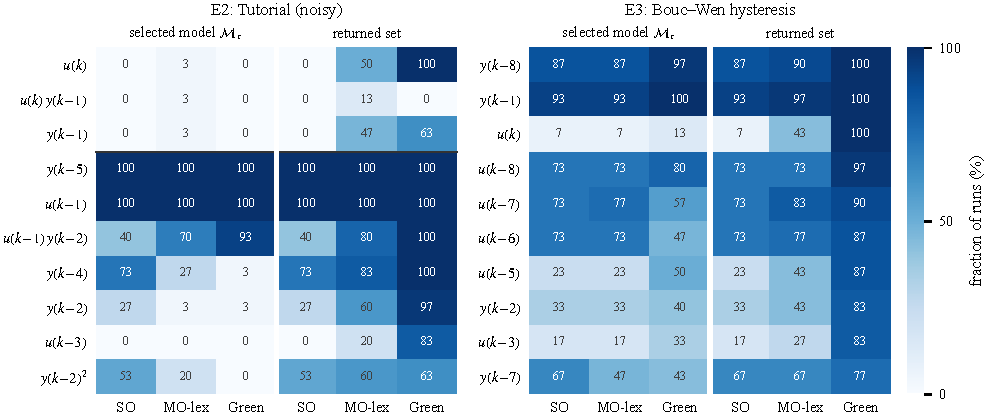
\includegraphics[width=\textwidth]{figures/fig_regressors.pdf}
\caption{Percentage of the \nSeeds{} runs with $\rho=1$ in which each regressor appears in the selected model
$\mathcal M_\tau$ (left block of each panel) and in at least one model of the returned set (right block), for the ten
most frequent regressors. On E2, the three regressors above the line form the true structure \eqref{eq:tutorial}.}
\label{fig:regressors}
\end{figure}

\begin{figure}[t]
\centering
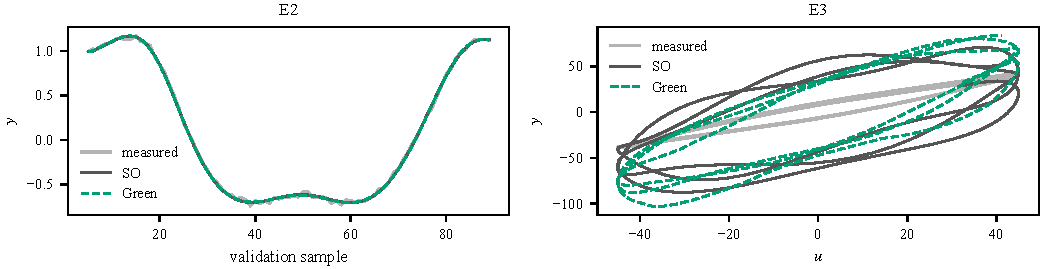
\includegraphics[width=\textwidth]{figures/fig_freerun.pdf}
\caption{Free-run validation of the selected models of the representative runs with $\rho=1$: E2 time series (left)
and E3 input--output loop (right).}
\label{fig:freerun}
\end{figure}

\subsection{Sensitivity to the selection tolerance}
The tolerance $\tau=\tauSel$ was fixed before the experiments; Fig.~\ref{fig:tau} examines how the selected models
change when it varies between $0$ and $1$, without altering the reported results. In agreement with
Proposition~\ref{prop:tau}(ii), the selected cost of the Pareto-based configurations decreases monotonically with
$\tau$, whereas SO is unaffected because it returns a single model. The range of costs that Green MGGP offers is much
wider: on E3, its median selected cost falls from $14$ operations at $\tau=0.05$ to $4$ at $\tau\ge0.5$, while that of
MO-lex stays at or above $16$. The price is a gradual increase in validation error, from $0.078$ to $0.082$ on E3 and
from $0.031$ to $0.032$ on E2. At $\tau=0.1$ on E2, the median selected cost equals $\Ctrue$, but equality of cost does not imply equality of structure. Models at this cost omit the true bilinear regressor; the \ECRecTauGreenApB\% of Green runs that recover all true regressors select more expensive models. Recovery is therefore not monotone in $\tau$. The
dotted lines show the smallest validation error available in the Green sets: on E2 and E3 it is below the median
validation error of the selected model of every configuration, which confirms that the sets contain better models than
any rule based on identification data alone can identify.

\begin{figure}[t]
\centering
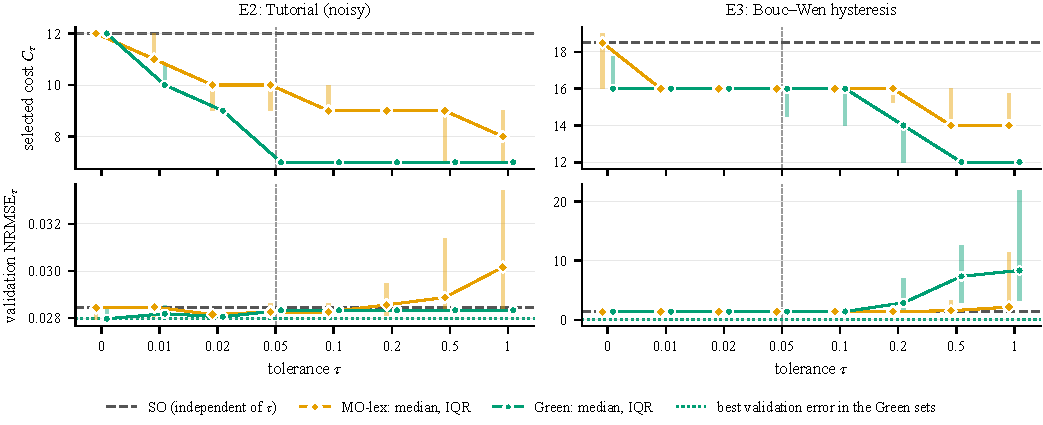
\includegraphics[width=\textwidth]{figures/fig_tau.pdf}
\caption{Sensitivity of the $\tau$-rule with $\rho=1$ on E2 and E3 (on E1 the selected model does not depend on
$\tau$): median (markers) and interquartile range (bars) over \nSeeds{} runs of the selected cost (top) and of its
free-run validation NRMSE (bottom) for MO-lex and Green MGGP. The dashed horizontal line is SO, which returns a single
model; the vertical dashed line marks the declared value $\tau=\tauSel$, and the dotted line is the median of the
smallest validation error in the Green sets.}
\label{fig:tau}
\end{figure}

\subsection{Effect of the multiplication weight}\label{sec:rho}
All configurations were also run with the bit-level weight $\rho_K$, which reproduces the Green-Box complexity up to
the factor $B$ (Proposition~\ref{prop:rescaling}); those runs reproduced bit for bit an earlier set of runs with the
complexity $B\,a+B^{\alpha}b$, and the SO runs, which do not use the cost, were identical under both weights.
Table~\ref{tab:rho} summarises the comparison. The conclusions on the selection scheme do not depend on the weight:
under $\rho_K$, Green MGGP again exceeds both baselines in identification and validation hypervolume in every run
($A_{12}=1.00$), with medians of \RhoEBKaraGreenHVid, \RhoECKaraGreenHVid{} and \RhoEDKaraGreenHVid{} against at most
\RhoEBKaraLexHVid, \RhoECKaraLexHVid{} and \RhoEDKaraLexHVid, and its selected models are \RhoEBKaraCostRed\%,
\RhoECKaraCostRed\% and \RhoEDKaraCostRed\% cheaper than those of SO in Karatsuba-weighted cost, against
\RhoEBOneCostRed\%, \RhoECOneCostRed\% and \RhoEDOneCostRed\% in operations under $\rho=1$.

\begin{table}[!htbp]
\centering
\caption{Effect of the multiplication weight $\rho$ over 30 runs (medians). HV: identification hypervolume; $\Delta C_\tau$: reduction of the median selected cost of Green MGGP relative to SO, with the cost of the same scenario; $a{+}b$ and $C_{\rho_K}$: operation count and Karatsuba-weighted cost of the selected Green model; same: fraction of seeds in which Green MGGP selects the same structure under both weights.}
\label{tab:rho}
\setlength{\tabcolsep}{3.5pt}
\small
\begin{tabular}{llccccccc}
\toprule
 & & \multicolumn{3}{c}{HV$_\mathrm{id}$} & & \multicolumn{2}{c}{Green $\mathcal M_\tau$} & \\
\cmidrule(lr){3-5}\cmidrule(lr){7-8}
Ex. & weight & SO & MO-lex & Green & $\Delta C_\tau$ & $a{+}b$ & $C_{\rho_K}$ & same \\
\midrule
E1 & $\rho=1$ & 0.640 & 0.829 & 0.896 & 22\% & 7 & 48.6 & 100\% \\
 & $\rho_K$ & 0.738 & 0.884 & 0.929 & 20\% & 7 & 48.6 &  \\
\midrule
E2 & $\rho=1$ & 0.508 & 0.702 & 0.878 & 42\% & 7 & 48.6 & 80\% \\
 & $\rho_K$ & 0.622 & 0.773 & 0.910 & 43\% & 7 & 48.6 &  \\
\midrule
E3 & $\rho=1$ & 0.736 & 0.798 & 0.955 & 14\% & 16 & 109.5 & 0\% \\
 & $\rho_K$ & 0.819 & 0.874 & 0.969 & 14\% & 16 & 109.5 &  \\
\bottomrule
\end{tabular}
\end{table}


Fig.~\ref{fig:ab} locates the selected models in the plane of additions and multiplications. Lines of constant $C_1$
have slope $-1$, whereas lines of constant $C_{\rho_K}$ are almost horizontal, so that under $\rho_K$ a structure is
cheaper essentially when it has fewer multiplications, whatever its number of terms, while under $\rho=1$ terms and
degrees are exchanged one for one. On E1 and E2 the Green selections under both weights concentrate on the same point,
$(a,b)=(4,5)$ and $(4,6)$, below and to the left of all SO selections. On E3 they spread over the lattice, from three
to eight terms, and the most frequent selection differs between the weights, $(5,9)$ for $\rho=1$ and $(6,10)$ for
$\rho_K$, whereas the SO models use seven or eight terms and between $10$ and $17$ multiplications.

\begin{figure}[t]
\centering
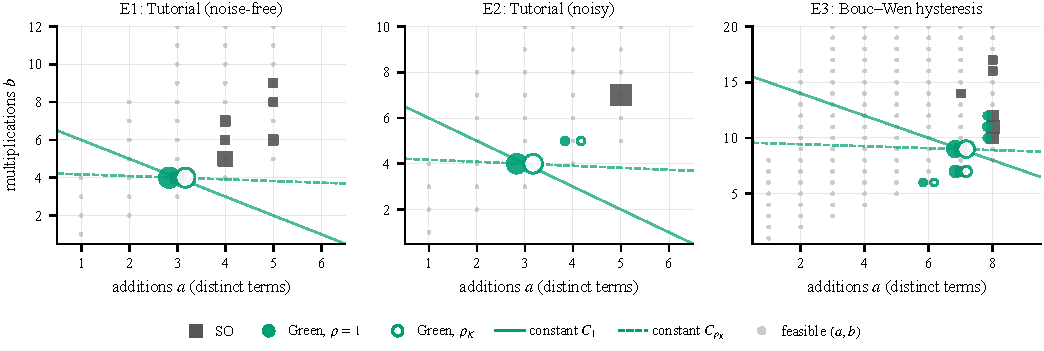
\includegraphics[width=\textwidth]{figures/fig_ab.pdf}
\caption{Selected models in the plane of additions $a$ and multiplications $b$ over \nSeeds{} runs: SO, and Green MGGP
with $\rho=1$ and with $\rho_K$ (marker area proportional to the number of runs; the two Green weights are offset
horizontally for visibility). Grey dots are the feasible pairs counted by $L(G,h)$ in Proposition~\ref{prop:cost}; the
lines pass through the most frequent Green selection with constant $C_1$ (solid) and constant $C_{\rho_K}$ (dashed).}
\label{fig:ab}
\end{figure}

The weight does change which structures are selected. On E1 the same structure is selected under both weights in every
run, but on E2 this holds in \RhoECSame\% of the runs and on E3 in only \RhoEDSame\%. With $\rho=1$, adding a linear term
costs as much as raising the degree of an existing one, whereas with $\rho_K$ a multiplication costs about eleven
additions, so the two weights favour different shapes of polynomial. On E3 the models selected with $\rho=1$ need
\RhoEDOneGreenOps{} operations per sample against \RhoEDKaraGreenOps{} for those selected with $\rho_K$, and they are also
cheaper when costed with $\rho_K$ (\RhoEDOneGreenKar{} against \RhoEDKaraGreenKar), at a higher median validation error
(\EDGreenVALsel{} against \KaraEDGreenVALsel). Because the identified structures depend on $\rho$, the weight is a
property of the target platform that should be set before identification; Section~\ref{sec:energy} shows that, on the
platform used here, measured execution supports $\rho=1$ rather than $\rho_K$.

\subsection{Computational effort and limitations}
The median run times of Green MGGP were \EBGreenTime, \ECGreenTime{} and \EDGreenTime~s, comparable to those of SO
(\EBSOTime, \ECSOTime{} and \EDSOTime~s) and lower than those of MO-lex (\EBLexTime, \ECLexTime{} and \EDLexTime~s); the
extra sorting is negligible compared with model evaluation. These are software timings of the identification
procedure; the time and energy needed to execute the identified models are examined separately in
Section~\ref{sec:energy}. The study is also bounded by the package itself. Besides the backshift requirement above, its
simulation routines fail for products of delayed outputs and inputs whenever the maximum delay exceeds one, so such
individuals receive infinite error in all three configurations; these failures are also the source of the ties that
break the hypothesis of Theorem~\ref{thm:lex}. A further implementation error affects output factors at the largest delay: the circular output buffer can substitute $y(k-1)$ for the intended delayed output, as detailed in Section~\ref{sec:method}. Consequently, some stored simulation errors are not errors of the intended polynomial. The selected models are numerically unaffected within the reported simulator agreement, but this does not establish that the returned sets or search trajectories are unaffected. All methods use the same predictor; correcting it would require repeating the searches. The present results therefore characterise this implementation and its restrictions.
The generation counts are equal, but Green produces more offspring per generation; equal-evaluation comparisons remain future work. Pareto trade-offs between accuracy and complexity are already central to multigene symbolic regression in GPTIPS~\cite{Searson2015}, and complexity objectives in symbolic regression extend to the order of nonlinearity~\cite{VSH2009}. The present comparison concerns the operation cost of the duplicate-free polynomial and its treatment by the selection scheme. An ablation with Pareto selection and term or node count is still needed to isolate the contribution of the arithmetic objective from the selection scheme. Finally, the examples are small, and
the classification mode, which returns a single objective, was not considered.
